\chapter{Обзор существующих подходов решения задачи поиска активного}
\label{section_module}

Существует много методов решения задачи поиска активного модуля, они в основном
отличаются математической формулировкой задачи и подходами ее решения.
Рассмотрим наиболее популярные из них.





\section{Формальная постановка задачи поиска активного модуля}

В этой работе рассматривается задача поиска активного модуля, для которой
существует различные подходы решения.  Все решения основаны на анализе
экспресси гена совместно с регуляторными сетями, в которых узлами являлись
гены, а ребрами -- их возможные взаимодействия. Под анализом экспресси гена
обычно подразумевается его \emph{P}-значение анализа дифференциальной
экспрессии.

Если формально описать, то у нас есть связный неориентированный граф $G = (V,
E)$ и весовая функция (\emph{P}-значения) на вершинах $w: V \to [0, 1]$.
Существует также неизвестный связный подграф (\emph{активный или функциональный
модуль}) и $M$ набор вершин этого подграфа.  Веса $w$ считаются такими
случайными числами, что веса вершин из $M$ -- независимые одинаково
распределенные и следуют <<сигнальному>> распределению, а веса вершин из $V
\setminus M$ -- независимые одинаково распределенные, но следуют <<шумовому>>
распределению.  Здесь считается, что веса соответствуют \emph{P}-значению
статистического теста, где для вершин из $V \setminus M$ выполняется нулевая
гипотеза, и соответствующие веса следуют равномерному распределению $U(0, 1)$.
Согласно~\cite{Dittrich2008a}, веса вершин из $M$ следуют бета-распределению
$B(a, 1)$ для некоторого параметра $a$.

Таким образом, формально решаемая задача:
\begin{problem}
    Пусть $G=(V, E)$ -- связный неориентированный граф с весовой функцией
    $\omega : V \to [0, 1].$ $M$ -- неизвестный связный подграф (активный
    модуль) в графе $G.$ Веса в вершинах из $M$ из бета-распределения $B(a,
    1),$ в остальных вершинах веса из равномерного распределения $U(0, 1).$
      Найти активный модуль $M$.
\end{problem}





\section{Поиск активного модуля с помощью алгоритма имитации отжига}

Авторы статьи~\cite{Ideker2002} являются одними из первых, кто предложил выделять
активные регуляторные модули.  Они предложили подход, оценивающий важность
подсети. Зная \emph{P}-значения каждого индивидуального гена, считались
значения обратной функций распределений стандартного нормального распределения
$z_i = F^{-1}(1 - p_i).$

Чтобы получить совместное \emph{z}-значение $z_A$ для всей подсети $A$ из $k$
генов, суммировались $z_i$ по всем генам в подсети:
\begin{equation}\label{eq:zA}
z_A = \frac{1}{\sqrt{k}}\sum_{i \in A} z_i.
\end{equation}
Подсети всех размеров сравнимы по этой системе подсчета: если все $z_i$ из
стандартного нормального распределения, то и $z_A$ также будут стандартно
нормально распределены, не зависимо от размера подсети $k$.  Высокое значение
$z_A$ соответствует биологически важным активным модулям.

Чтобы правильно зафиксировать связь между экспрессией и топологией сети,
надо определить, является ли оценка $z_A$ подсети более высокой чем ожидаемая
относительно случайного набора генов. Произвольно проецируется множество генов
размера $k$ с использованием подхода Монте-Карло, вычисляются их оценки $z_A$,
а затем они используются для получения оценки среднего значения $\mu_k$ и
стандартного отклонения $\sigma_k$ для каждого $k.$ Поскольку ожидается, что
средние и стандартные отклонения будут гладкой функцией по $k,$ можно уменьшить
шум в оценках Монте-Карло, используя среднее скользящее окно. Используя эти
оценки, скорректированный вес подсети $s_A$ считается как:
\[s_A = \frac{z_A - \mu_k}{\sigma_k}.\]

Требовалось найти подсеть с максимальной оценкой $z_A,$ но это задача является
\emph{NP}-трудной, в связи с чем авторы использовали для поиска таких подсетей
метод отжига~\cite{Kirkpatrick1983}. Так же авторами было разработано несколько
эвристик. Решатель с предложенным подходом решения этой задачи доступен в виде
плагина \emph{jActiveModules} для программы
\emph{Cytoscape}~\cite{Shannon2003}.

Этот подход применялся много раз для метаболических моделей
в~\cite{Patil2005,Mardinoglu2013,Mardinoglu2015}.





\section{Эвристические методы поиска активного модуля}

В~\cite{Rajagopalan2005} авторы предложили новый метод оценки важности подсети
на основе~\cite{Ideker2002}.  Для подсети $A$ из $k$ генов функция оценки
подсети считается по формуле:
\[z_A = \frac{\sqrt{k}}{\sigma} \frac{\sum_{i}{C_i}}{k},\]
где $\sigma$ -- стандартное отклонение распределения $z_i$ весов и $C_i$
-- скорректированный вес гена.  Эта формула была получена из оригинальной
формулы \eqref{eq:zA} путем апроксимации значений $\mu$ математического
ожидания и $\frac{\sigma}{\sqrt{k}}$ стандартного отклонения случайного
множества $k$ генов из полного распределения $z$ весов.

Скорректированный вес считается по формуле:
\[C_i = z_i - max(\beta \mu, z^EP_i),\]
где $\beta$ - эмпирический параметр для контроля доли генов с положительными
весами и $z^EP_i$ - величина, по которой нахождения соседа у $i$-го гена
с маленьким \emph{P}-значением зависит от степени вершины.

Эвристический алгоритм, предложенный авторами~\cite{Rajagopalan2005}, состоит из
следующих шагов:
\begin{enumerate}
    \item Построить связные подграфы из генов положительного веса $C_i.$
    \item Выбирать ранее не рассмотренный подграф и запустить \emph{DFS}
        ограниченной глубины $d$ из смежных для подграфа вершин. Если
        достигли другого связного подграфа, объединить их и добавить новый
        подграф, если оценка не хуже оценки компонент.
    \item Построить новые подграфы с помощью удаления вершин не точек
        сочленений, что позволит увеличить оценку.
\end{enumerate}

Основное время выполнения этого алгоритма занимает второй шаг. Поэтому во всех
экспериментах авторы запускали алгоритм с $d=2$, что существенно снижает
пространство поиска и время работы алгоритма.





\section{Формулировка через сведение к задаче поиска связного подграфа
максимального веса}
В работе~\cite{Dittrich2008a,Beisser2010} авторы предложили другую
математическую формулировку задачи поиска активного модуля.  В этой работе
рассматривается модель максимального правдоподобия, где для каждого гена
определяется правдоподобие принадлежности его активному модулю из данных
дифференциальной экспрессии.  Точно так же как в задаче~\cite{Ideker2002},
в этой задаче надо максимизировать правдоподобия подсети, что эквивалентно
задачи \emph{MWCS}.

Следуя~\cite{Pounds2003} распределение \emph{P}-значений рассматривается как
смесь бета-распределения $B(a, 1)$ и равномерного распределения
\(\mathcal{U}(0, 1)\), что хорошо соответствует наблюдаемым данным (как
например в рисунке~\ref{fig_dittrich2008}).  Авторы предложили назвать это
\emph{смесью бета-равномерного} (\emph{beta-uniform mixture}, \emph{BUM})
распределения.  Предполагается, что бета-распределение соответствует сигналу,
а равномерное -- шуму.  Также авторы предложили метод оценки $a$ и долю
шума с помощью максимального правдоподобия.

\begin{figure}
    \centering
    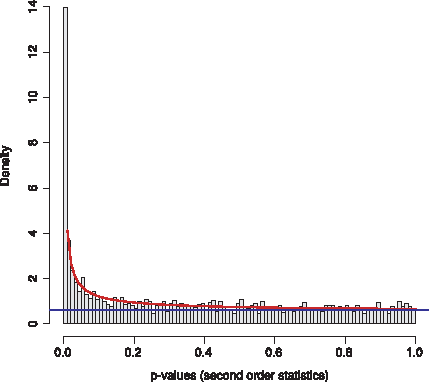
\includegraphics{dittrich2008.pdf}
    \caption{Пример гистограммы \emph{P}-значений и плотности
        соответствующего бета-равномерного распределения
    \label{fig_dittrich2008}}
\end{figure}

По аналогии с тестом, отношения правдоподобия веса одного гена для
\emph{P}-значения $p_i$ определяется по формуле:
\[ S(p_i) = \log \left(\frac{B(a, 1)(p_i)}{\mathcal{U}(0, 1)(p_i)}\right)
= \log a + (a -1)\log p_i.\]
Как указано в~\cite{Pounds2003}, модель смеси \emph{BUM} позволяет оценить
ожидаемую долю ложных отклонений (\emph{False Discovery Rate}, \emph{FDR}). Из
этого вычисляется пороговое \emph{P}-значение $\tau(FDR)$, которое контролирует
\emph{FDR} для положительно оценивающих \emph{P}-значений. Таким образом, мы
получаем скорректированную оценку логарифмического отношения правдоподобия,
\[ S^{FDR}(p_i) = \log\Big(\frac{ap_i^{a-1}}{a\tau^{a-1}}\Big) = (a
- 1)\Big( \log p_i - \log \big(\tau(FDR)\big)\Big).\]

Вес подграфа считается как сумма весов $S^{FDR}(p_i)$ отдельных генов. Поиск
активного модуля -- модуля с максимальным весом -- соответствует задаче
\emph{MWCS}.

Несмотря на то, что эта задача является \emph{NP}-трудной, авторы предлагают
решатель, который сможет найти оптимально доказуемое или хорошее решение за
приемлемое время. Авторы сводят задачу \emph{MWCS} к другой \emph{NP}-трудной
задаче -- задаче \emph{PCST} (\emph{Prize Collecting Steiner Tree}). Затем,
с помощью решателя~\cite{Ljubic2006} достаточно точно решается экземпляр
\emph{PCST}. Авторами был предложен решатель \emph{heinz} для задачи
\emph{MWCS}.

В конце работы авторы предлагают сравнения с методом \emph{jActiveModules}
и показывают, что сведение к задаче \emph{MWCS} позволяет значительно лучше
и стабильнее находить активные модули на модельных данных.

\begin{figure}
    \centering
    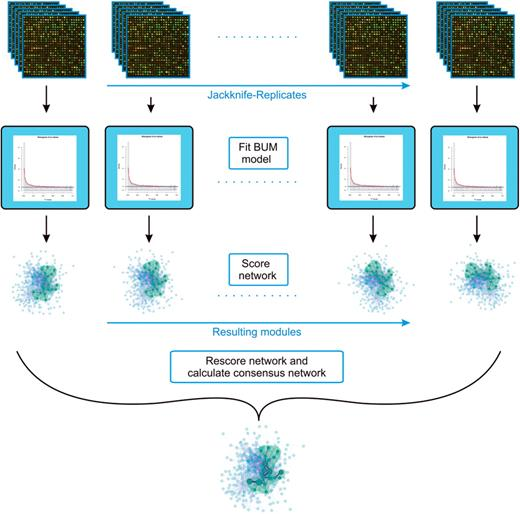
\includegraphics[width=3.0in]{consensus.jpeg}
    \caption{
        Схема консенсусного метода.  Сначала данные микрочипа повторно
        дискретизируются.  Дифференциальная экспрессия вычисляется на всех
        образцах \emph{jackknife}.  Из распределения $P$-значений оцениваются
        параметры BUM распределения, и на их основе расчитываются веса вершин.
        Для каждой сети вычисляется \emph{MWCS}. Этот набор модулей впоследствии
        используется для получения консенсусных значений вершин и ребер.  Затем
        исходная сеть переоценивается с помощью консенсусных значений.  В конце
        консенсусный модуль вычисляется как \emph{MWCS} размера исходного модуля.
    }
    \label{consensus}
\end{figure}

В~\cite{Beisser2012} авторы исследуют точность и надежность трех известных
методов поиска активного модуля, касающихся:
1) интегрированных данных экспрессии генов и
2) сетевой структуры самой сети \emph{белок-белковых взаимодействий}
   (\emph{Protein-Protein Interaction}, \emph{PPI}).  В результате
   исследования, авторы предлагают новый метод расчета точных и надежных
   модулей, вводя новую концепцию \emph{консенсусных модулей}.  Для оценки
   надежности функциональных модулей в интегрированном сетевом анализе, авторы
   используют метод повторной дискретизации (resampling) \emph{кулачковый нож}
   (\emph{delete-half jackknife}). Он используется для повторной выборки
   входных данных микрочипа и построения набора результирующих модулей.
   В процедуре повторной дискретизации \emph{delete-half jackknife} $50\%$ наблюдений
   отбрасываются случайным образом, и на основе оставшихся наблюдений считается
   дифференциальная экспрессия.  Консенсусный модуль суммирует полученные
   модули как один очень точный и надежный модуль со значениями поддержки на
   его вершинах и ребрах, которые определяют их надежность
   (рисунок~\ref{consensus}).

В работе~\cite{Beisser2012} авторы представили новую версию решателя
\emph{heinz}.  В решателе \emph{heinz2} появилась возможность включения веса
ребер и установления размера искомого активного модуля.

%\section{Другие подходы к постановке задачи активного
%модуля}

%Кроме перечисленных выше, существуют и другие подходы к определению и
%поиску активного модуля.
%
%В ~\cite{McClellan2013} предлагается метод \emph{NetWeAvers}. В нем
%также рассматривается список индивидуальных \emph{P}-значений для всех
%генов и регуляторная сеть межгенных взаимодействий. В этой сети с
%помощью алгоритма \emph{Walktrap}~\cite{Pons2005}, использующего модель
%случайных блужданий, выполняется поиск сильно-связных модулей. Поиск
%происходит без учета \emph{P}-значений. После выделения модулей
%выполняется их оценка с использованием среднего или медианного
%\emph{P}-значений в модуле. Статистическая значимость оценивается с
%помощью перестановочного теста. Концептуально, можно сказать, что в этом
%методе сначала независимо от экспериментальных данных из сети выделяются
%потенциальные функциональные наборы генов, которые затем анализируются
%по типу анализа представленности.
%
%Другой подход предложен в методе
%\emph{KeyPathwayMiner}~\cite{Alcaraz2012}. В нем формулируется задача
%поиска наибольшего модуля, содержащего не больше заданного числа слабо
%регулируемых, «исключительных», генов. Так же, как \emph{MWCS}, эта
%задача является \emph{NP}-трудной. Авторами было предложено несколько
%алгоритмов для ее решения, два неточных: жадный и муравьиный алгоритмы,
%и один точный алгоритм на основе метода ветвей и границ. Отметим, что
%точный алгоритм работал за приемлемое время только для небольших
%значений числа «исключительных» генов. В~\cite{Alcaraz2014} тем же
%коллективом метод был расширен для поддержки нескольких типов данных. В
%этом случае, на модуль ставилось одновременно несколько ограничений по
%числу исключительных узлов по разным типам данных. К серьезным
%недостаткам этого метода можно отнести сложность выбора параметров
%алгоритма.

\section{Постановка цели и задач диссертации}
Для большинства существующих методов решения задачи поиска активного модуля
ответом является некоторый связный подграф заданного графа. Примерами таких
методов являются описанные
ранее~\cite{Ideker2002,Dittrich2008a,Alcaraz2012,Sergushichev2016}.  Общей
проблемой этих методов является необходимость выбора некоторого порога
значимости. При этом, если, например, ослабить такой порог, то размер решения
увеличится за счет добавления новых вершин, но некоторые вершины могут
и пропасть (например, как на рисунке \ref{fig:consistency}). Такое поведение
особенно неудобно с точки зрения пользователя, и усложняет интерпретируемость
результатов.
\begin{figure}
    \begin{subfigure}{.45\textwidth}
        \centering
        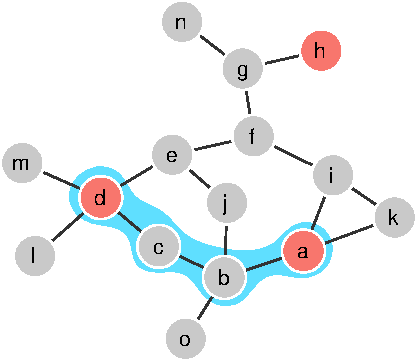
\includegraphics{new-consistency4.pdf}
        \caption{строгий порог\\поиск подграфа размера $4$}
    \end{subfigure} %
    \begin{subfigure}{.45\textwidth}
        \centering
        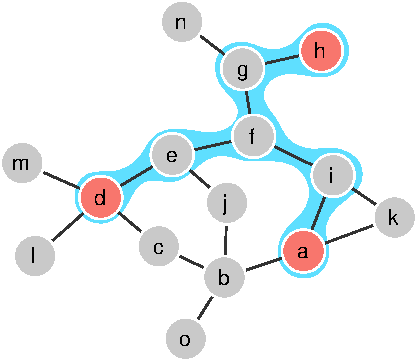
\includegraphics{new-consistency7.pdf}
        \caption{слабый порог\\поиск подграфа размера $7$}
    \end{subfigure}
    \centering
    \caption{
        Вероятно важные вершины и вершины, о которых мало, что известно покрашены
        в красный и серый цвет соответственно.  Синим цветом выделен значимый
        подграф при заданном пороге.  В панелях требуется найти значимый
        подграф заданного размера с максимальным количеством важных вершин.
        Рисунок иллюстрирует несоответствия решений с разными порогами, то есть
        в решение задачи со слабым пороговым значением не входят все вершины из
        решения со строгим пороговым значением.
    }
    \label{fig:consistency}%
\end{figure}

Целью работы является разработатка метода мягкой классификации вершин.

Задачами диссертационной работы являются:
\begin{itemize}
    \item Разработать метод монотонно-связного ранжирования.
    \item Разработать метод оценки вероятностей принадлежности вершины в активный модуль.
\end{itemize}




\chapterconclusion
Таким образом, мы описали задачу поиска активного модуля, существующие подходы решения,
а так же проблемы, возникающие при таких подходах решения этой задачи.

